
\documentclass[12pt,a4paper]{scrartcl}

\usepackage[a4paper, left=2cm, right=1cm, bottom=1cm, top=1cm, includeheadfoot]{geometry}
\usepackage[ngerman]{babel}
\usepackage[utf8]{inputenc} % comment this if you uncomment utf8x
%\usepackage[utf8x]{inputenc} % uncomment this if there are problems with 'ä', 'ü', 'ö'
\usepackage{ucs}
\usepackage[usenames,dvipsnames]{xcolor}
\usepackage[fleqn]{amsmath}
\usepackage{amsfonts}
\usepackage{amssymb}
\usepackage{color}
\usepackage{listings}
\usepackage{hyperref}
\usepackage{amsfonts}
\usepackage{listings}
\usepackage{scrpage2}
\usepackage{graphicx}


\definecolor{mygray}{rgb}{0.9,0.9,0.9}
\lstset{language=[Visual]Basic, morekeywords={param, local}}


\lstset{
   literate={ö}{{\"o}}1
           {ä}{{\"a}}1
           {ü}{{\"u}}1
           {ß}{{\ss}}1
           {é}{{\'e}}1,
   inputencoding=ansinew,
   extendedchars=true,
   basicstyle=\scriptsize\ttfamily,
   numberstyle=\scriptsize,
   breaklines=true,
   tabsize=2,
   numbersep=5pt
}
\lstdefinestyle{customcpp}{
   language=C++,
   backgroundcolor=\color{mygray},
   numbers=left,
   keywordstyle=\color{blue}\bfseries,
   stringstyle=\color{BrickRed}\ttfamily,
   commentstyle=\color{OliveGreen}\ttfamily,
   showspaces=false,
   showstringspaces=false,
   showtabs=false
}
\lstdefinestyle{customoutput}{
   backgroundcolor=\color{mygray},
   numbers=none,
   showspaces=false,
   showtabs=false
}

\newcommand{\sourceCode}[1]{\lstinputlisting[style=customcpp]{#1}} %beinhaltet alle benötigten Packages etc.
\begin{document}
\graphicspath{{./}}

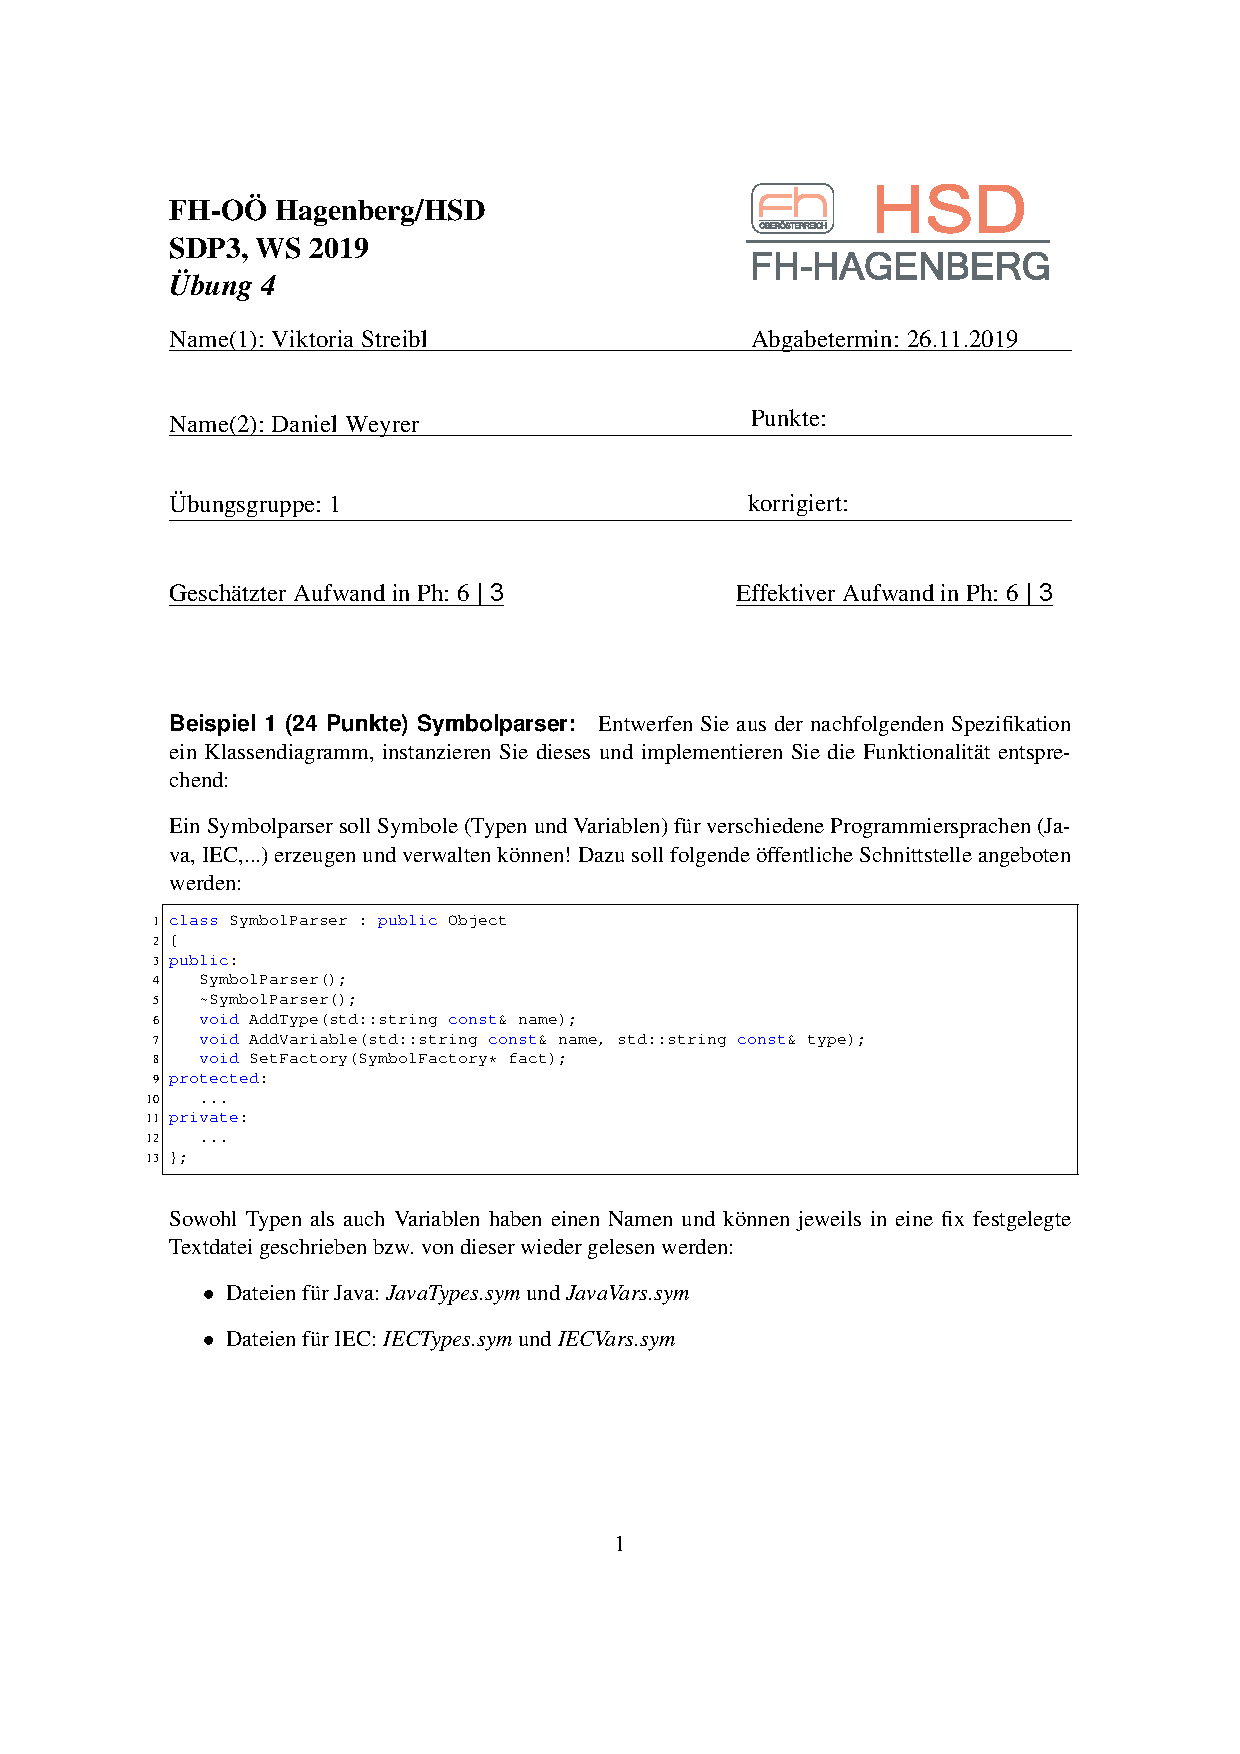
\includepdf[pages=-]{Angabe.pdf}

\title{SDP - Exercise 04} % Übungsname und Nummer angeben
\subtitle{winter semester 2019/20} % Semester angeben oder auskommentieren, falls nicht erwünscht
\author{
Viktoria Streibl - S1810306013\\
  Daniel Weyrer - S1820306044
} % Autorenname
\date{\today} % Das heutige Datum automatisch einfügen

\maketitle % Titelseite erstellen

\newpage
\tableofcontents % Inhaltsverzeichnis erstellen
\newpage

\ihead{Viktoria Streibl}
\ohead{Daniel Weyrer}
\chead{SDP3-UE Uebung 04}

\section{Organizational}
\subsection{Team}
\begin{itemize}
	\item Viktoria 	Streibl 		- 	S1810306013
	\item Daniel 	Weyrer		-	S1820306044
\end{itemize}

\subsection{Roles and responsibilities}
\subsubsection{Jointly}
\begin{itemize}
	\item Planning
	\item Documentation
	\item Systemdocumentation
	\item Class Diagram
\end{itemize}

\subsubsection{Viktoria Streibl}
\begin{itemize}
	\item Class SymbolFactory
	\item Class IECSymbolFactory
	\item Class JavaSymbolFactory
	\item Documentation	
\end{itemize}

\subsubsection{Daniel Weyrer}
\begin{itemize}
	\item Documentation
	\item TestDriver	
	\item Class SymbolParser
	
\end{itemize}

\subsection{Effort}

\subsubsection {Viktoria Streibl}
\begin{itemize}
	\item estimated: 6 ph 
	\item actually: 6 ph
\end{itemize}

\subsubsection {Daniel Weyrer}
\begin{itemize}
	\item estimated: 3 ph 
	\item actually: 3 ph
\end{itemize}

\section{Requirenment Definition(System Specification)}


\section{System Design}
\subsection{Classdiagram}
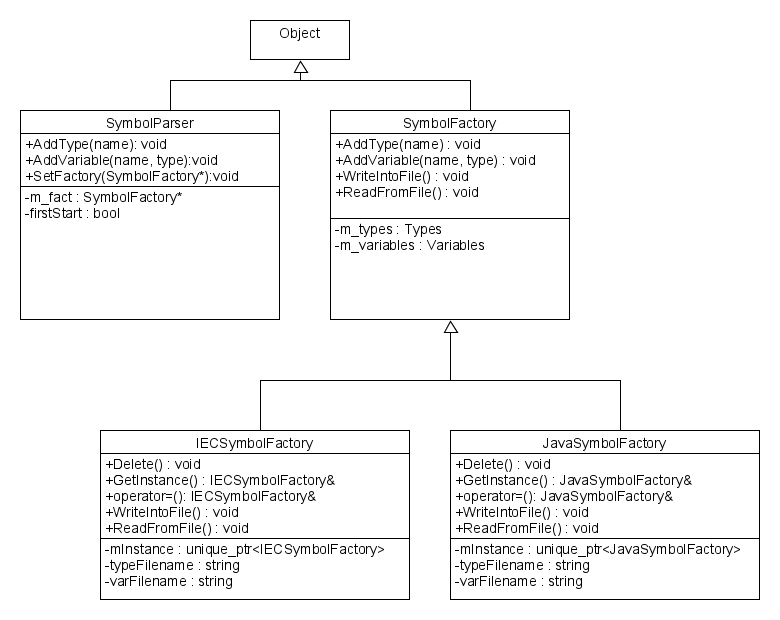
\includegraphics[scale=0.65]{ClassDiagramm}

%\subsection{Design Decisions}
%\subsubsection{}

\newpage
\section{Component Design}
\subsection{SymbolParser}
\begin{itemize}
	\item AddType
	\subitem Calls the AddType of SymbolFactory
	\item AddVariable
	\subitem Calls the AddVariable of SymbolFactory
	\item ReadFile
	\subitem Reads the files and adds all existing types and variables
	\item SetFactory
	 \subitem Gets the current language and sets it as current factory. Calls ReadFile at the first call
\end{itemize}



\subsection{SymbolFactory}
\begin{itemize}
	\item AddType
	\subitem Gets the type and adds to the others if it's not exists.
	\item AddVariable
	\subitem Gets the variable name and adds to the others. It checks if it is the first variable-name of this type.
	\item WriteIntoFile
	\subitem Virtual Method to write all types ad variables back into the file
	\item ReadFromFile
	 \subitem Virtual Method to read all types and variables of a file
\end{itemize}

\subsection{IECSymbolFactory}
Is a Singleton Class.
\begin{itemize}
	\item AddType
	\subitem Gets the type and adds to the others if it's not exists.
	\item AddVariable
	\subitem Gets the variable name and adds to the others. It checks if it is the first variable-name of this type.
	\item WriteIntoFile
	\subitem Writes all types and variables into the iec files.
	\item ReadFromFile
	 \subitem Reads from the iec-files and save all types and variables into the programm.
\end{itemize}

\subsection{JavaSymbolFactory}
Is a Singleton Class.
\begin{itemize}
	\item AddType
	\subitem Gets the type and adds to the others if it's not exists.
	\item AddVariable
	\subitem Gets the variable name and adds to the others. It checks if it is the first variable-name of this type.
	\item WriteIntoFile
	\subitem Writes all types and variables into the java files.
	\item ReadFromFile
	 \subitem Reads from the java-files and save all types and variables into the programm.
\end{itemize}

\subsection{TestDriver}
The Testdriver test alle functions of the clients. It tests the interface for the Epos-Company as well as the NortelNetwork-Company. It encrypt and decrypt several files. It contains also some functions:
\begin{itemize}
	\item Adds Types and Variables of Java and IEC
	\item Tests what happens to add a Variable but no existing Type
	\item Tests to read the Files and a new Variable
	\item Tests to add existing Type 
\end{itemize}

\newpage
\section{Test Protocol}

\subsection{Testfiles}
\subsubsection{IECTypes.sym}
\sourceCode{./SymbolParser/SymbolParser/IECTypes.sym}
\subsubsection{IECVars.sym}
\sourceCode{./SymbolParser/SymbolParser/IECVars.sym}

\subsubsection{JavaTypes.sym}
\sourceCode{./SymbolParser/SymbolParser/JavaTypes.sym}
\subsubsection{JavaVars}
\sourceCode{./SymbolParser/SymbolParser/JavaVars.sym}

%\subsection{ConsoleOutput}
%\sourceCode{./SymbolParser/SymbolParser/ConsoleOutput.txt}

\newpage
\section{Source Code}

\subsection{SymbolParser}
\subsubsection{SymbolParser.h}
\sourceCode{./SymbolParser/SymbolParser/SymbolParser.h}
\subsubsection{SymbolParser.cpp}
\sourceCode{./SymbolParser/SymbolParser/SymbolParser.cpp}
\newpage

\subsection{SymbolFactory}
\subsubsection{SymbolFactory.h}
\sourceCode{./SymbolParser/SymbolParser/SymbolFactory.h}
\newpage
\subsubsection{SymbolFactory.cpp}
\sourceCode{./SymbolParser/SymbolParser/SymbolFactory.h}
\newpage

\subsection{IECSymbolFactory}
\subsubsection{IECSymbolFactory.h}
\sourceCode{./SymbolParser/SymbolParser/IECSymbolFactory.h}
\subsubsection{SymbolFactory.cpp}
\sourceCode{./SymbolParser/SymbolParser/IECSymbolFactory.h}
\newpage

\subsection{JavaSymbolFactory}
\subsubsection{JavaSymbolFactory.h}
\sourceCode{./SymbolParser/SymbolParser/JavaSymbolFactory.h}
\newpage
\subsubsection{JavaSymbolFactory.cpp}
\sourceCode{./SymbolParser/SymbolParser/JavaSymbolFactory.h}
\newpage



\subsection{TestDriver}
\subsubsection{TestDriver.cpp}
\sourceCode{./SymbolParser/SymbolParser/TestDriver.cpp}
\newpage
% Um Quellcode einzufügen einfach diesen Befehl verwenden:
%\sourceCode{Relativer/Pfad/zum/SourceCode.Endung}

\end{document}